%%%%%%%%%%%%%%%%%%%%%%%%%%%%%%%%%%%%%%%%%%%%%%%%%%%%%%%%%%%%%%%%%%%%%%%%%%
\documentclass[11pt,a4j]{jarticle}
%%%%%%%%%%%%%%%%%%%%%%%%%%%%%%%%%%%%%%%%%%%%%%%%%%%%%%%%%%%%%%%%%%%%%%%%%%
\usepackage{amsmath}
%\usepackage{graphicx}% Include figure files
\usepackage[dvipdfmx]{graphicx}
\usepackage{txfonts}
\usepackage{bm}% bold math
\usepackage{float}
\usepackage{here}
\usepackage{array}
\usepackage{cases}
\usepackage[T1]{fontenc}
\usepackage{etoolbox}
\usepackage[top=20truemm,bottom=20truemm,left=25truemm,right=25truemm]{geometry}%余白
\usepackage{layout}
\usepackage{wrapfig}
\usepackage{indentfirst}
\usepackage[hang,small]{caption}
%\usepackage[subrefformat=parens]{subcaption}
\usepackage[dvipdfmx]{color}
\captionsetup{compatibility=false}
%\renewcommand{\indent}{\hspace*{1zw}}
\renewcommand{\abstractname}{} 
\renewcommand{\figurename}{Fig.}
\renewcommand{\tablename}{Table.}
\renewcommand{\thefootnote}{\fnsymbol{footnote}}
\pagestyle{plain}
%%%%%%%%%%%%%%%%%%%%%%%%%%%%%%%%%%%%%%%%%%%%%%%%%%%%%%%%%%%%%%%%%%%%%%%%%%
\makeatletter%% プリアンブルで定義する場合は必須
\patchcmd{\maketitle}{\@fnsymbol}{\@alph}{}{}  % Footnote numbers from symbols to small letters
\long\def\@makecaption#1#2{% \@makecaption を再定義します
  \vskip\abovecaptionskip
  \iftdir\sbox\@tempboxa{#1\hskip1zw#2}%
    \else\sbox\@tempboxa{#1~ #2}% ここの : を ~ に変更する
  \fi
  \ifdim \wd\@tempboxa >\hsize% 
    \iftdir #1\hskip1zw#2\relax\par
      \else #1~ #2\relax\par\fi% ここの : を ~ に変更する
  \else
    \global \@minipagefalse
    \hbox to\hsize{\hfil\box\@tempboxa\hfil}% センタリング
%   \hbox to\hsize{\box\@tempboxa\hfil}%      左詰め
%   \hbox to\hsize{\hfil\box\@tempboxa}%      右詰め
  \fi
  \vskip\belowcaptionskip}


 \DeclareRobustCommand\cite{\unskip
\@ifnextchar[{\@tempswatrue\@citex}{\@tempswafalse\@citex[]}}
 \def\@cite#1#2{$^{[\hbox{\scriptsize{#1\if@tempswa , #2\fi}]}}$}
 \def\@biblabel#1{[#1]}
\makeatother%% プリアンブルで定義する場合は必須
\setlength{\columnsep}{8  truemm}
\setlength{\linewidth}{81 truemm} 
%%%%%%%%%%%%%%%%%%%%%%%%%%%%%%%%%%%%%%%%%%%%%%%%%%%%%%%%%%%%%%%%%%%%%%%%%%
\begin{document}
%%%%%%%%%%%%%%%%%%%%%%%%%%%%%%%%%%%%%%%%%%%%%%%%%%%%%%%%%%%%%%%%%%%%%%%%%%
\begin{titlepage}
%\begin{flushright}
%{\large
%指導教員(主査):〇〇〇〇 教授 \\ % 主査
%副査:□□□□ 教授                % 副査
%}
%\end{flushright}
\begin{center}
\vspace*{150truept}
{\huge マイクロスイマー2成分系のダイナミクス}\\ % タイトル
\vspace{10truept}
%{\huge }\\ % サブタイトル(なければコメントアウト)
\vspace{180truept}
{\huge 平成30年度}\\
\vspace{20truept}
{\huge 京都大学工学部工業化学科}\\ 
{\huge 化学プロセス工学コース}\\ 
{\huge 移動現象論研究室}\\ 
\vspace{50truept}
{\huge 堀米 厚志}\\ % 著者
\vspace{50truept}
%{\huge \today}\\ % 提出日
\end{center}
\end{titlepage}
%%%%%%%%%%%%%%%%%%%%%%%%%%%%%%%%%%%%%%%%%%%%%%%%%%%%%%%%%%%%%%%%%%%%%%%%%%
% 目次の表示
\thispagestyle{empty}
%\pagenumbering{}
\tableofcontents
\clearpage
\pagenumbering{arabic}
\section{緒言}
\subsection{研究背景}
%\subsubsection{}
\par アクティブマターの自走現象は,非平衡系システムの性質を研究する上で最も重要な研究分野のひとつである.特に生物学において自走現象はよく認知されており,マクロスケールでは人間を含むすべての生物に自走現象が認められることはもちろん,ミクロスケールにおいてもモータータンパク質\cite{myosin,dynein}など数多くの例がある.さらには,非生物系においても水中における油滴の自走現象\cite{oil}など,多くの分野にて自走現象は報告されている.また,自走現象を伴うアクティブマターには,集団運動の際に単体の性質からは予測できない特異性を示すことがあることが知られている.マクロスケールでは魚や鳥が大きな群れをなして泳ぐ様子が観測されることがあり\cite{fish},ミクロスケールにおいてもバクテリアの集団渦運動\cite{uzu}を始めとした例が多く挙げられる.このように,自走現象はアクティブマター単体の性質のみならず,その集団運動の性質を記述するにも極めて重要な現象である.
\par ミクロスケールにおいて,自走現象が認められる物質を「自走粒子」と呼ぶ.その中でも,バクテリアやヤヌス粒子などに代表されるような周辺流体との流体力学的相互作用によって自己推進する「マイクロスイマー」は,工学的応用に富んだ物質として非常に注目を集めている.生活習慣病のひとつである歯周病の原因として有名なバイオフィルムの構造解析\cite{film}やドラッグデリバリーシステムへの応用\cite{DDS}など,マイクロスイマーの動的挙動を理解することで得られる工学的応用例は数知れない.このような工学的システムにおいて,マイクロスイマーはある種の拘束空間内に存在しており,このような拘束空間はマイクロスイマーの集団行動に強い影響を及ぼすことが示されている\cite{C}.しかしながら,考慮すべき流体力学的相互作用の複雑性より,流体力学的相互作用を完璧に考慮した解析を行うことは到底不可能であり,行うにしても莫大な計算コストがかかる.そのため,これまで流体力学的相互作用を無視するか遠方界近似にて考慮するかなど簡易化された研究が専ら\cite{hydro}であり,拘束空間にて流体力学的相互作用を考慮した研究は,本研究室で行われた先行研究以外ではほとんど行われていない\cite{oyama}.そのため,拘束空間を考慮した研究を行うことは極めて優位性が高いといえる.
\par マイクロスイマーは,自己推進する際に周辺流体に発生する生成流によって3種類に分類され\cite{squirmer},マイクロスイマーの集団運動の性質はその分類への依存性が高いことが知られている.まず,粒子の推進方向に対して周辺流体に伸長流を生成する「Pusher型」が挙げられる.生物学的な実例を考えると,Pusher型マイクロスイマーには,生物後方に持っている繊毛を用いて生物後方の流体をさらに後方に押しやることで推進するバクテリアがある.逆に,粒子の推進方向に対して周辺流体に収縮流を生成するのは「Puller型」と呼ばれる.この型には,生物の前方にある繊毛を用いて生物前方の流体を生物後方に押しやることで推進するバクテリアがある.最後の分類は「Neutral型」と呼ばれ,もともとある流速場によって推進する.Neutral型には,全身に広がる繊毛をよく動かしてもともとある流速場に沿って推進するバクテリアが例として挙げられる.これまでのマイクロスイマーにおける集団行動の研究では,これらのうちの単成分系に着目した研究が大半であった.マイクロスイマーに限らずアクティブマター多成分系に着目した研究は少ないが,多種間のバクテリア集団\cite{ex1}や捕食-被食関係にある生物間システムダイナミクス\cite{ex2}など実用的な例は数多く見られる.そのため,マイクロスイマー多成分系のダイナミクスについて解析することは,マイクロスイマーを工学的に応用するにおいて,そのさらなる発展に寄与することが期待される.
\par 以前に本研究室で行われた先行研究においては,以上のことを踏まえて,拘束空間内におけるマイクロスイマー各成分の単成分系ダイナミクスの解析が行われた\cite{oyama}.先行研究では,拘束空間内において,マイクロスイマーの泳動形態を示すパラメーター$\alpha$に関して$0<\alpha<1$を満たすPuller型マイクロスイマーでのみ,体積分率やシステムサイズに関わらず,常に進行波のような集団運動が観測されることが報告された(Fig.\ref{oyama}).そこで本研究では,マイクロスイマー多成分系の中でもPusher型/Puller型2成分系に着目し,その拘束空間内での挙動を解析することで,Puller型マイクロスイマーによって発生する進行波の系全体の集団運動に及ぼす影響を調べることを目的とした.
\begin{figure}[h]
\begin{center}
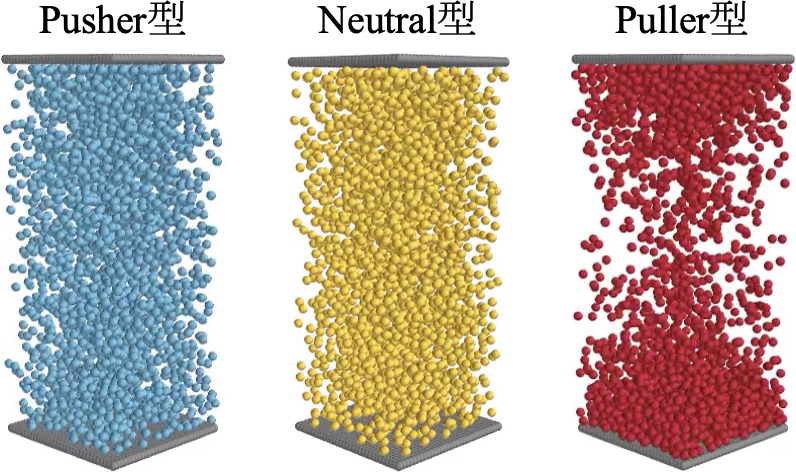
\includegraphics[width=100mm]{./images/previoswork.png}
\caption{拘束空間内における各成分のスナップショット}
\label{oyama}
\vspace{0truemm}
\end{center}
\end{figure}

\subsection{研究概要}
\par 本研究では,マイクロスイマーPusher型/Puller型2成分系のダイナミクスについて定量的な解析を行うため,直接数値計算を行った.まず,計算コストを削減するために,マイクロスイマーのモデルとして後述するSquirmerモデルを採用し,それをSmoothed Profile Method(SPM)\cite{SPM}に組み込んでシミュレーションを行った.シミュレーションの際には,コロイドシミュレーターKAPSELを用いた.そして,シミュレーションを結果を定量的に解析するために局所数密度自己相関関数と局所組成変動自己相関関数を計算し,拘束空間内の粒子の運動が定常状態になった後における局所数密度と局所組成変動のゆらぎについて考察することで,各々の平均組成依存性を調べた.

%%%%%%%%%%%%%%%%%%%%%%%%%%%%%%
%%%%%%%%%%%%%%%%%%%%%%%%%%%%%%
\newpage
\section{計算手法}
\subsection{Squirmerモデル}
\par マイクロスイマーのモデルとして「Squirmerモデル」\cite{Lighthill,Blake}を採用した.このモデルは球状粒子モデルで,泳動形態を表現するために粒子表面における流体の流速場を境界条件として設定したものである.
%\par マイクロスイマーのモデルとして「Squirmerモデル」を採用した.このモデルは球状粒子モデルで,泳動形態を表現するために粒子表面における粒子と流体の速度差を境界条件を設定したものである\cite{13-14}.
\begin{equation}
  \boldsymbol{u}^s = \sum_{n=1}^\infty\frac{2}{n(n+1)}B_n P_n^\prime(\cos{\theta}) \sin{\theta}\hat{\boldsymbol{\theta}}
       \label{boundary1}
 \end{equation}
\noindent
ここで$\boldsymbol{r}$は粒子の中心からその表面上の点に向かう単位ベクトルであり,$\theta$は$\boldsymbol{r}$と粒子の推進方向$\boldsymbol{e}$との間の極角,$\boldsymbol{\theta}$は単位極角ベクトルである.$\boldsymbol{u}^s$は粒子表面における流体の流速場,$B_n$は各Fourier係数,$P_n^\prime$は$n$次Legendre多項式の導関数である.しかし,実際の直接数値計算では式(\ref{boundary1})の最初の2つの項しか保持されない.
\begin{equation}
       \boldsymbol{u}^s = B_1\left(\sin{\theta} + \frac{\alpha}{2}\sin{2\theta}\right)\hat{\boldsymbol{\theta}}
       \label{boundary2}
 \end{equation}
\noindent
ここで,Fourier第一係数$B_1$は孤立粒子の遊泳速度の大きさ($U_0 =\displaystyle\frac{2}{3}B_1$)を与え,Fourier第二係数$B_2$は粒子が流体に及ぼす剪断応力を与える.この2つの係数を利用して,粒子の分類は$\alpha =B_2/B_1$の符号により決定される.$\alpha<0$では周辺流体に伸長流を生成するPusher型,$\alpha>0$では収縮流を生成するPuller型,$\alpha=0$では潜在的な流場で遊泳するNeutral型となる.
\begin{figure}[h]
\begin{center}
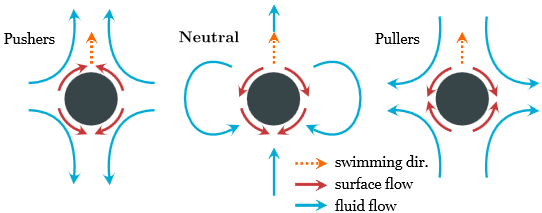
\includegraphics[width=100mm]{./images/squirmer_2.png}
\caption{SquirmerモデルにおけるPusher型,Neutral型,Puller型の概略図\cite{oyama}}
\label{squirmer}
\vspace{0truemm}
\end{center}
\end{figure}

\subsection{Navier-Stokes方程式}
\par 流体$\boldsymbol{u}_{\rm{f}}$への支配方程式として,非圧縮条件下で一定粘性率$\eta$のNavier-Stokes方程式を使用する.
\begin{align}
      \boldsymbol{\nabla}\cdot{\boldsymbol{u}}_{\rm{f}}&=0
	   \\
      \rho_{\rm f}\left(\partial_t+{\boldsymbol{u}}_{\rm{f}}\cdot\boldsymbol{\nabla}\right){\boldsymbol{u}}_{\rm{f}}&=\boldsymbol{\nabla}\cdot\boldsymbol{\sigma}_{\rm{f}}
\end{align}
\label{Navier_Stokes}
\noindent
ここで,$\rho_{\rm f}$は流体の質量密度,$\boldsymbol{\sigma}_{\rm{f}}$は応力テンソルである.応力テンソルは等方性圧力項及び剪断応力項$\boldsymbol{\sigma}_{\rm{f}}^\prime$からなる.
\begin{align}
   \boldsymbol{\sigma}_{\rm{f}}&=-p\boldsymbol{I}+\boldsymbol{\sigma}_{\rm{f}}^\prime
      \\
   \boldsymbol{\sigma}_{\rm{f}}^\prime&=\eta[\boldsymbol{\nabla}{\boldsymbol{u}}_{\rm{f}}+(\boldsymbol{\nabla}{\boldsymbol{u}}_{\rm{f}})^t]
\end{align}
\label{sigma}
\noindent
ここで$\boldsymbol{I}$は単位テンソルである.

\subsection{Newton-Euler方程式}
\par 粒子$i$の位置,速度及び角速度は$\boldsymbol{R}_{\rm{i}}$,$\boldsymbol{V}_{\rm{i}}$及び$\boldsymbol{\Omega}_{\rm{i}}$と表される.粒子の時間発展はNewton-Euler方程式で与える.
\begin{align}
   \dot{\boldsymbol{R}}_i &= \boldsymbol{V}_i , & \dot{\boldsymbol{Q}}_i &= \text{skew}(\boldsymbol{\Omega}_i)\cdot \boldsymbol{Q}_i
      \\
   M_{\text{p}}\dot{\boldsymbol{V}}_i &= \boldsymbol{F}_i^{\text{H}}+\boldsymbol{F}_i^{\text{C}} , & \boldsymbol{I}_{\text{p}}\cdot\dot{\boldsymbol{\Omega}}_i &= \boldsymbol{N}_i^{\text{H}}
\end{align}
\label{Newton_Euler}
\noindent
ここで,$\boldsymbol{Q}_i$は回転行列,$M_{\text{p}}$は粒子の質量,$\boldsymbol{I}_{\text{p}}$は慣性モーメント,$ \text{skew}(\boldsymbol{\Omega}_i)$は式(\ref{skew})で表される$\boldsymbol{\Omega}_i$の対称行列である.
\begin{equation}
  \text{skew}(\boldsymbol{\Omega}) =
       \begin{pmatrix}
          0&-\Omega_3&\Omega_2\\
          \Omega_3&0&-\Omega_1\\
          -\Omega_2&\Omega_1&0
       \end{pmatrix},\ \ \
       \boldsymbol{\Omega}=
       \begin{pmatrix}
          \Omega_1\\
          \Omega_2\\
          \Omega_3
       \end{pmatrix}
       \label{skew}
 \end{equation}
流体から受ける力$\boldsymbol{F}_i^{\text{H}}$及びトルク$\boldsymbol{N}_i^{\text{H}}$は,以下のように表される.
\begin{align}
   \boldsymbol{F}_i^H&=\int_{\boldsymbol{S}_i}\text{d}\boldsymbol{S}_i\cdot \boldsymbol{\sigma}_{\rm{f}}\\
   \boldsymbol{N}_i^H&= \int_{\boldsymbol{S}_i}\left( \boldsymbol{r}-\boldsymbol{R}_i \right) \times\left(\text{d}\boldsymbol{S}_i\cdot\boldsymbol{\sigma}_{\rm{f}}\right)
\end{align}
\label{FandN}
粒子間の直接的相互作用による力$\boldsymbol{F}_i^{\text{C}}$は,体積拘束分が切り捨てられたLennard-Jones $2n-n$ポテンシャル($n = 18$)より与えられる.
\begin{align}
   \boldsymbol{F}_i^{\rm C}&=\sum_j\boldsymbol{F}_{ij} ,\quad \boldsymbol{F}_{ij}=-\boldsymbol{\nabla}_iU\left( r_{ij}\right), \\
   U\left(r_{ij}\right)&= 
      \begin{cases} 
         4\epsilon\left[\left(\cfrac{\sigma}{r_{ij}}\right)^{36}- \left(\cfrac{\sigma}{r_{ij}}\right)^{18}\right]+\epsilon &\left( r_{ij}\le 2^{1/18}\sigma\right)\\ 
         0 &\left( r_{ij}\ge 2^{1/18}\sigma\right) 
      \end{cases}
\end{align}
ここで$\boldsymbol{F}_{ij}$は粒子$i$と粒子$j$との間の相互作用ポテンシャルに起因して粒子$i$に及ぼされる力,$\boldsymbol{\nabla}_i$は粒子$i$の座標に関する空間微分,$r_{ij}=|\boldsymbol{R}_j - \boldsymbol{R}_i|$は2つの粒子間距離,$\sigma$は粒子の直径,$\epsilon$はシステム内エネルギー単位である.

\subsection{Smoothed Profile Method(SPM)}
\par コロイドシミュレーターKAPSELでは,流体及び粒子の方程式を効率的に解くためにSPM(Smoothed Profile Method)\cite{SPM}を採用している.この方法では,高価な計算コストをもたらす粒子と流体間の境界面の代わりに有限幅$\xi$の拡散界面を導入し,固体領域で1,流体領域で0,拡散界面内で連続的に変化する界面関数$\phi_{\rm{p}}$が全粒子に与えられ,その重ね合わせによって物理量が表される.本研究では,特に全流速場にこの界面関数が適用される.
\begin{equation}
  \boldsymbol{u} = (1-\phi_{\rm{p}})\boldsymbol{u}_{\rm{f}}+\phi_{\rm{p}}\boldsymbol{u}_{\rm{p}}
       \label{eq_u}
 \end{equation}
ここで$\boldsymbol{u}$は全流速場,$(1-\phi_{\rm{p}})\,\boldsymbol{u}_{\rm{f}}$,$\phi_{\rm{p}}\boldsymbol{u}_{\rm{p}}$はそれぞれ流体と粒子の流速場である.したがって,Navier-Stokes方程式は以下のように修正される.
\begin{align}
      \boldsymbol{\nabla}\cdot{\boldsymbol{u}}&=0
	   \\
      \rho_{\rm f}\left(\partial_t+{\boldsymbol{u}}\cdot\boldsymbol{\nabla}\right){\boldsymbol{u}}&=\boldsymbol{\nabla}\cdot\boldsymbol{\sigma}+\rho_{\rm f}\left(\phi_{\rm{p}}\boldsymbol{f}_{\rm{p}}+\boldsymbol{f}_{\rm{sq}}\right)
\end{align}
\label{Navier_Stokes}
ここで$\phi_{\rm{p}}\boldsymbol{f}_{\rm{p}}$は粒子の剛直性を保証する力,$\boldsymbol{f}_{\rm{sq}}$は流体と粒子間の速度差を生じさせる力である.

%%%%%%%%%%%%%%%%%%%%%%%%
%%%%%%%%%%%%%%%%%%%%%%%%
\newpage
\section{シミュレーション結果}
\par 本研究では先行研究においてPuller型粒子が進行波を生じた結果を再現するため,以下の条件を設定した.
\begin{enumerate}
\item Squirmer粒子の直径$\sigma$と拡散界面厚さ$\xi$はそれぞれ$\sigma=4\Delta$と$\xi=2\Delta$\ ($\Delta$は単位長さ).
\item 式(\ref{boundary2})のパラメーターである$B_1$は$B_1=0.375$,$\alpha$についてはPuller型では$\alpha=0.5$,Pusher型では$\alpha=-0.5$.
\item 体積分率$\psi$は$\psi=0.13$.
\item 粘性率$\eta$と流体質量密度$\rho_{\rm{f}}$をともに1,単位時間を$\rho_{\rm{f}}\Delta^2/\eta$.これにより,孤立Squirmer粒子のReynolds数$Re^0=\rho_{\rm{f}}U_0 \sigma/\eta$は1に設定される.
\item 外力は作用せず,浮力ははたらかない.
\end{enumerate}
ここで先行研究より,Puller型粒子の影響で発生する進行波のダイナミクスは$0<\alpha<1$を満たすPuller型粒子では体積分率$\psi$やシステムサイズに依存しないことが報告されている\cite{oyama}.そのため,本研究においては$\alpha$と$\psi$を固定して計算を行った.
\par さて,システムサイズが$64\Delta\times160\Delta\times64\Delta$のシステムでシミュレーションを行った(Fig.\ref{snapshot}).このシステムは$x$方向と$z$方向には周期的であるが,$y$方向には$y=1\Delta$と$y=159\Delta$の位置にある2つの平行壁に挟まれている.壁は2048個ある直径$4\Delta$の球状粒子で構成されており,初期の位置と向きから移動及び回転ができないように固定されている.Squirmer粒子の初期位置及び初期方向はランダムとした.Puller型粒子の組成$x_1$を変えてシミュレーション行い,壁からの距離の関数として局所数密度$\rho$の時間発展を計算した結果をFig.\ref{Rho}に示した.ここで,1,2はそれぞれPuller型,Pusher型を示す.$W(\ =160\Delta)$は$y$方向のシステムサイズ,$T_0$は全計算時間,$\rho_0$は平均数密度である.これより,$x_1=1$から考えて,Puller型粒子の組成が高いときにはPuller型粒子単体のときと同様に明瞭な進行波が生じるが,$x_1=0.7$付近で急激に進行波が弱まり,$x_1=0.6$付近で進行波が消失することが確認された.Puller型粒子の組成に比例して進行波が強まること自体は想定していた通りであったが,進行波が初めて生じる組成は想定よりも高く,$x_1=0.8$から急激に進行波が明瞭化するのは非常に興味深い結果である.

\newpage
\vspace*{15truemm}
\begin{figure}[h]
\begin{center}
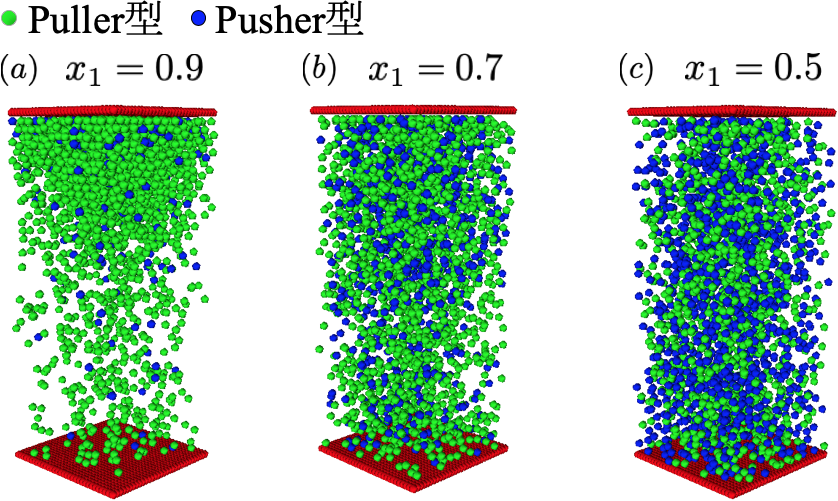
\includegraphics[width=110mm]{./images/snapshot.png}
\caption{シミュレーションスナップショット}
\label{snapshot}
\vspace{0truemm}
\end{center}
\end{figure}

\begin{figure}[h]
\begin{center}
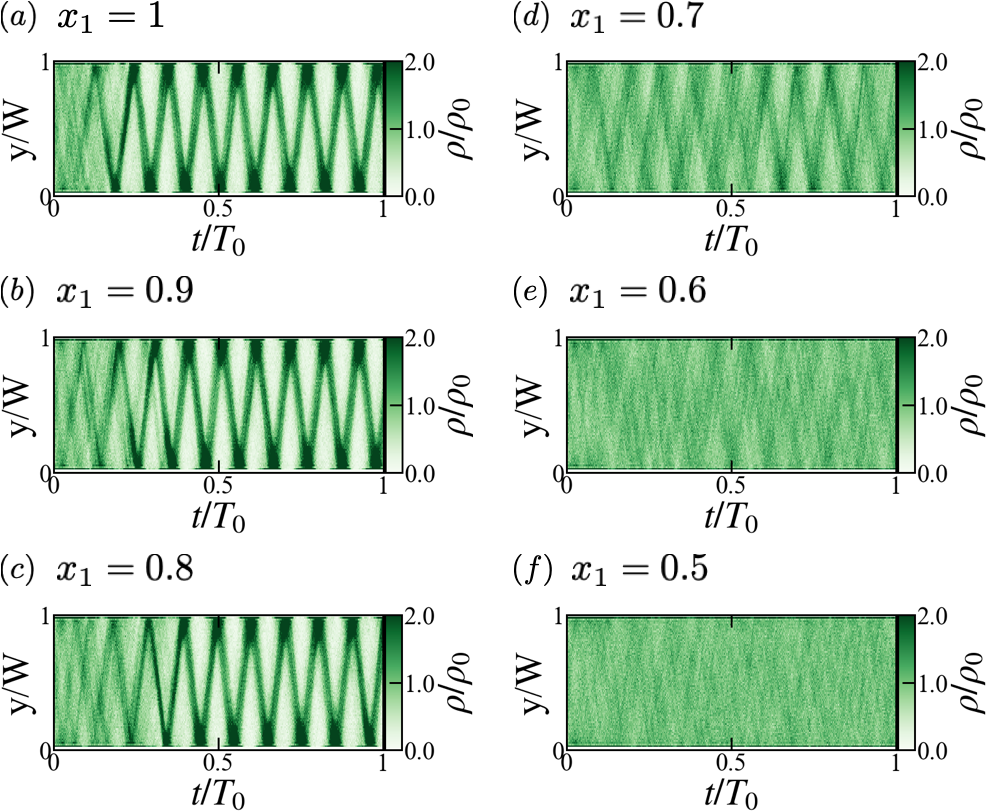
\includegraphics[width=120mm]{./images/y_t_rho.png}
\caption{各組成における局所数密度の時間発展}
\label{Rho}
\vspace{0truemm}
\end{center}
\end{figure}

%%%%%%%%%%%%%%%%%%%%%%%%%%%%%
%%%%%%%%%%%%%%%%%%%%%%%%%%%%%%
\newpage
\section{考察}
\subsection{進行波明瞭化組成}
\par 推進の際,Pusher型粒子は推進方向に対して伸長流を生成するのに対し,Puller型粒子は推進方向に対して収縮流を生成する.Puller型粒子を推進方向に対して無限に並べて運動させると,発生する収縮流のためにPuller型粒子同士が互いに引きつけ合い,推進方向の数密度変化が強化されることがシミュレーションで判明している\cite{oyama}.このことから,2成分系における数密度変化の時間発展を考察する.$x_1\approx 1$ではPusher型粒子の数密度変化への影響はほとんど考えられず,Puller型粒子同士による数密度変化の影響がシステム全体において非常に優位にはたらく.しかし,$x_1\approx 0.7$ではPusher型粒子が生成する伸長流の影響が強まることで推進方向の数密度変化が大幅に弱まり,Puller型粒子同士由来の数密度変化の影響がシステム全体において大幅に少なくなるのであると考えられる.
\vspace*{20truemm}
\begin{figure}[h]
\begin{center}
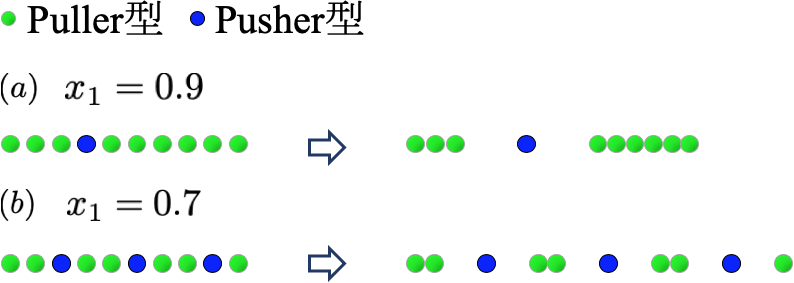
\includegraphics[width=120mm]{./images/wave_cause.png}
\caption{進行波明瞭化の定性的考察概略図}
\label{wave_cause}
\vspace{0truemm}
\end{center}
\end{figure}

%%%%%%%%%%%%%%%%%%%%%%%%%%%%%%
\newpage
\subsection{進行波速度}
\par Fig.\ref{Rho}に示された局所数密度の時間発展図には,その局所数密度により濃淡が現れている.その最も濃い部分の傾きは進行波の速度を表しているため,本章では局所数密度の時間発展図を用いて進行波速度の大きさを議論する.
\par まず,進行波がシステムの上下にある平行壁の位置に達したときの時間$t$をs測定した.測定方法としては,粒子の集団運動が定常状態となったことをFig.\ref{Rho}から判断し,その時間から先において局所数密度分布の偏りが最も大きくなった時間を図より読み取った.そこから,進行波が一方の壁から他方の壁に移る際の時間差$\ (=t_{n+1}-t_n)$を読み取り,進行波の速度の大きさを無次元化した量$\gamma_{\rm w}$を求めた.
\begin{equation}
  \gamma_{\rm w} = \displaystyle\frac{\delta(y/W)}{\delta(t/T_0)}=\displaystyle\frac{T_0}{t_{n+1}-t_n}
       \label{eq_c}
 \end{equation}
ここで,$\delta$は変化量を示す.$\gamma_{\rm w}$の各平均組成にて求めることで,平均組成依存性を解析することを目的とした.進行波が読み取れる組成範囲である$x_1=0.7〜1$における$\gamma_{\rm w}$を比較した結果をFig.\ref{velocity}に示す.これより,$\gamma_{\rm w}$は$\gamma_{\rm w}\approx  20$でほぼ一定であるという特性が現れた.したがって,進行波の速度の大きさはシステム内平均組成には依存しないことが示された.
\vspace*{20truemm}
\begin{figure}[h]
\begin{center}
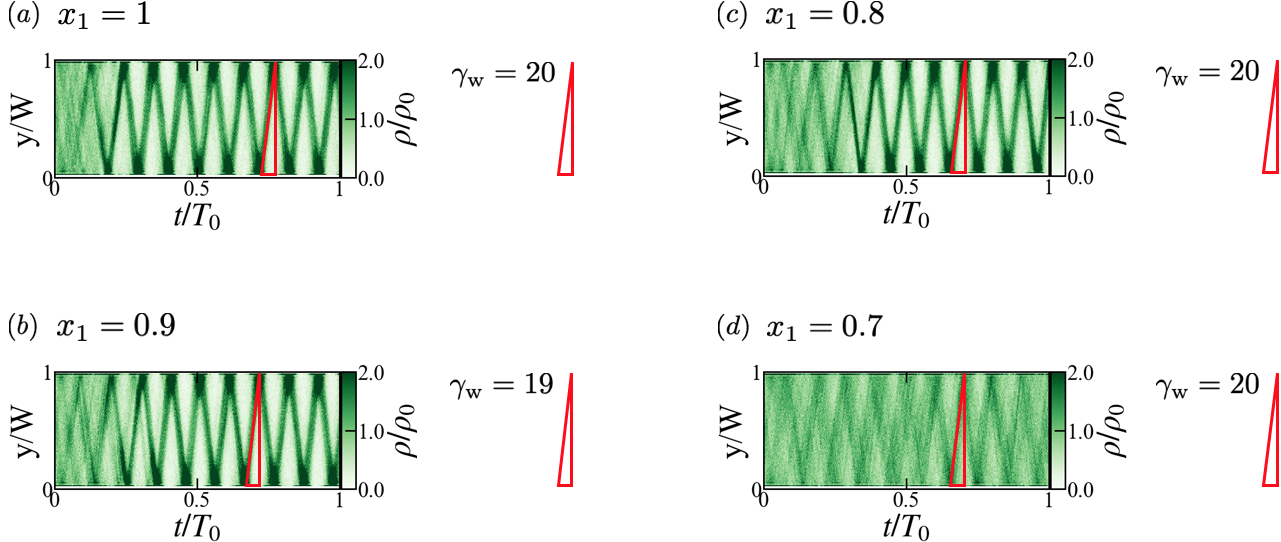
\includegraphics[width=150mm]{./images/gamma.png}
\caption{$\gamma_{\rm w}$の平均組成依存性}
\label{velocity}
\vspace{0truemm}
\end{center}
\end{figure}

%%%%%%%%%%%%%%%%%%%%%%%%%%%
\newpage
\subsection{局所数密度と局所組成変動のゆらぎ}
\par この章では,局所数密度$\hat\rho$と局所組成変動$\delta\hat X$のゆらぎを定量的に求める計算手法を示す,全粒子数$n$と組成変動$\delta X$を以下のように定義する.
\begin{align}
   n &= n_1+n_2
         \\
   \delta X &= \displaystyle\frac{1}{n}[x_2 n_1(\boldsymbol{r})-x_1 n_2(\boldsymbol{r})]
\label{yamamoto}
\end{align}
ここで$x$は平均組成,$\boldsymbol{r}$は相対位置ベクトルである.本研究では,ゆらぎを求める手法として自己相関関数に着目した.成分$\alpha$,$\beta$に対する局所粒子数の自己相関関数は以下で与える\cite{yamamoto}.
\begin{equation}
  \langle\hat n_{\alpha}(\boldsymbol{r})\hat n_{\beta}(\boldsymbol{0})\rangle = n_{\alpha}n_{\beta}g_{\alpha\beta}(\boldsymbol{r})+n_{\alpha}\delta_{\alpha\beta}\delta(\boldsymbol{r})
       \label{g}
 \end{equation}
ここで,$\textasciicircum$は物理量が局所的であることを示す.$g_{\alpha\beta}(\boldsymbol{r})(\ =g_{\beta\alpha}(\boldsymbol{r}))$はある成分$\alpha$の成分$\beta$に対する動径分布関数,$\delta_{\alpha\beta}$はKroneckerのデルタ,$\delta(\boldsymbol{r})$は$\boldsymbol{r}$におけるデルタ関数である.式(\ref{g})の右辺第2項はある粒子とその粒子自身との自己相関関数を示すため,本研究で調べる局所数密度・局所組成変動の自己相関関数には不要な項である.そのため不要項は排除し,本研究において局所数密度自己相関関数$g_{\rho}(\boldsymbol{r})$と局所組成変動自己相関関数$g_{\delta X}(\boldsymbol{r})$は以下で定義した.
\begin{align}
   g_{\rho}(\boldsymbol{r}) &= \displaystyle\frac{1}{n^2}\langle\hat n(\boldsymbol{r})\hat n(\boldsymbol{0})\rangle={x_1}^2 g_{11}(\boldsymbol{r})+{x_2}^2 g_{22}(\boldsymbol{r})+2x_1 x_2 g_{12}(\boldsymbol{r})
      \\
   g_{\delta X}(\boldsymbol{r}) &= \langle\delta\hat X(\boldsymbol{r})\delta\hat X(\boldsymbol{0})\rangle={x_1}^2 {x_2}^2[g_{11}(\boldsymbol{r})+g_{22}(\boldsymbol{r})-2g_{12}(\boldsymbol{r})]
\end{align}
ここで,局所数密度自己相関関数は定義化するにあたり,局所組成変動自己相関関数と次元が揃うように全粒子数で規格化している.
\par 局所数密度・局所組成変動自己相関関数は動径分布関数の重ね合わせで表現されるため,2つとも動径分布関数のピーク位置$r(\ =\sigma)$においてピーク値を得る.そこで,局所数密度・局所組成変動自己相関関数のそれぞれのピークにおけるPuller型粒子平均組成依存性を調べることによって,局所数密度と局所組成変動それぞれの自己相関を考察することができる.これにより,拘束空間内における進行波のダイナミクスを定量的に解析した.
%%%%%%%%%%%%%%%%%%%%%%%%%%%%%%%
\newpage
\subsubsection{局所数密度のゆらぎ}
\par 局所数密度自己相関関数のピークのPuller型粒子平均組成依存性を示したのがFig.\ref{Rho_yuragi},各成分における動径分布関数それぞれのピークのPuller型粒子平均組成依存性を示したのがFig.\ref{gab}である.Fig.\ref{Rho_yuragi}から$0.7\le x_1 \le 0.8$の範囲において,ピーク値の飛躍が生じていることが分かる.これについては,Fig.\ref{gab}においても,$x_1=0.7$までは値が連続的に変化しているのに対し,$0.7\le x_1 \le 0.8$において値が不連続的に上昇していることもこの結果を支持している.$0.7\le x_1 \le 0.8$という値は$\bf 3$において進行波が明瞭化した組成と一致していることから,進行波の明瞭化により局所数密度のゆらぎが生じたことが定量的に示されたと考えられる.
\vspace*{8truemm}
\begin{figure}[h]
\begin{center}
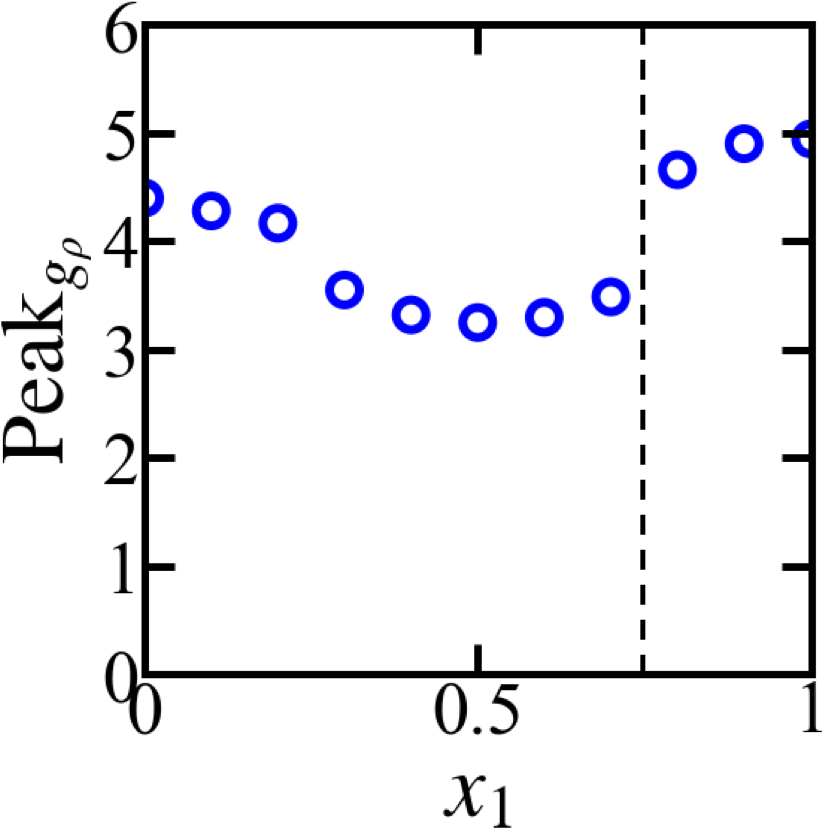
\includegraphics[width=70mm]{./images/Peak_rho.png}
\caption{局所数密度自己相関関数のピークの平均組成依存性}
\label{Rho_yuragi}
\vspace{0truemm}
\end{center}
\end{figure}
\vspace*{5truemm}
\begin{figure}[h]
\begin{center}
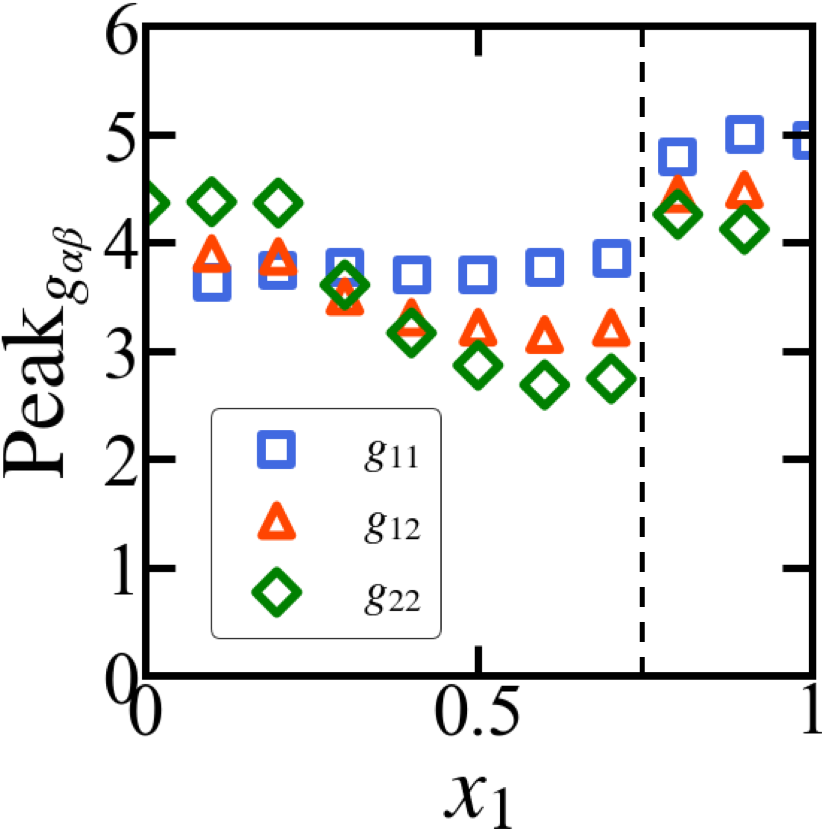
\includegraphics[width=70mm]{./images/Peak_g.png}
\caption{各成分における動径分布関数それぞれのピークの平均組成依存性}
\label{gab}
\vspace{0truemm}
\end{center}
\end{figure}
%%%%%%%%%%%%%%%%%%%%%%%%%%%%%%
\newpage
\subsubsection{局所組成変動のゆらぎ}
\par 局所組成変動自己相関関数のピークのPuller型粒子平均組成依存性を示したのがFig.\ref{X_yuragi}である.ピークは最大値でもオーダーが$10^{-2}$であり,極めて低い確率であることが分かる.これより,組成変動のゆらぎはほとんど発生しておらず,システム全体で各粒子成分は乱雑に混合していることが定量的に示された.

\vspace*{20truemm}
\begin{figure}[h]
\begin{center}
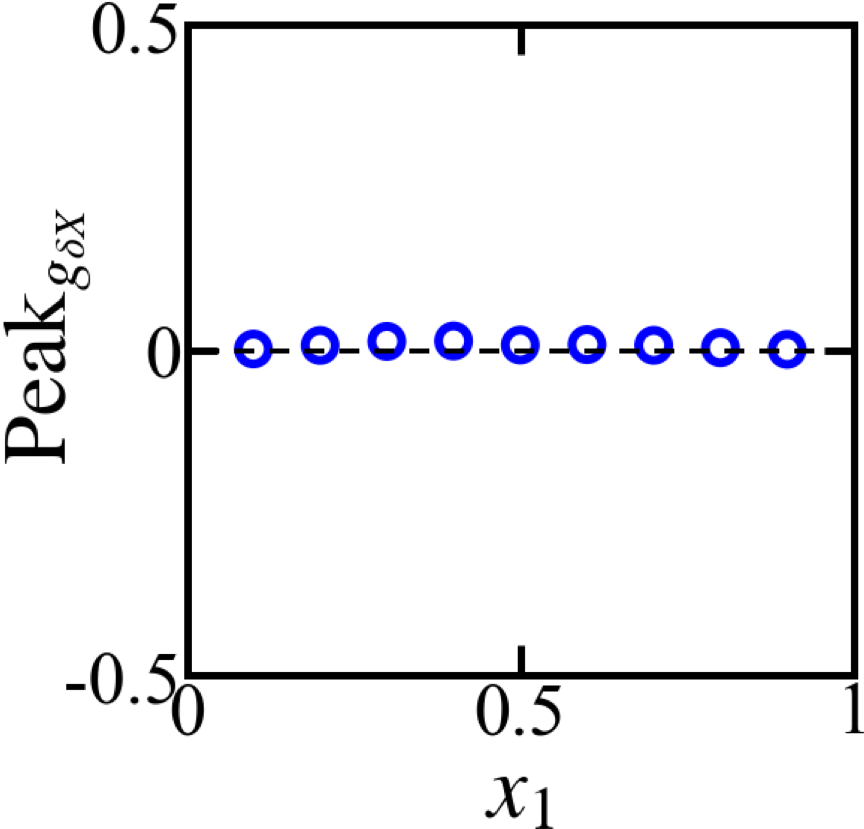
\includegraphics[width=70mm]{./images/Peak_X.png}
\caption{局所組成変動自己相関関数のピークの平均組成依存性}
\label{X_yuragi}
\vspace{0truemm}
\end{center}
\end{figure}

%%%%%%%%%%%%%%%%%%%%%%%%%%%%%
%%%%%%%%%%%%%%%%%%%%%%%%%%%%%%
\newpage
\section{結言}
\par 本研究では,拘束空間内におけるマイクロスイマーPusher型/Puller型2成分系の挙動を調べるため,コロイドシミュレーターKAPSELを用いた直接数値計算によるシミュレーションを行った.これにより,Puller型粒子組成が非常に高いときには拘束空間内で粒子は集団運動として進行波を発生させるが,$x_1=0.7$付近で急激に進行波が弱まり,$x_1=0.5$付近で進行波が消失することが観測された.しかし,その進行波の速度の大きさに関しては,進行波が発生するPuller型粒子組成範囲内において,進行波の速度の大きさは一定であることが示された.さらに,この挙動について定量的に解析するため局所数密度・局所組成変動自己相関関数を導入した結果,進行波の明瞭化に伴い局所数密度が大幅に変化すること,システム全体において,Puller型粒子とPusfer型粒子はいずれのPuller型粒子組成であっても常に乱雑に混合していることが定量的に示された.
\par 今後の課題としては,本研究では$x_1=0.7$付近で進行波の様相が急激に変化することの定量的な理由付けが不十分であったため,進行波の様相が変わる組成付近についてさらに詳細な解析を行い,その原因に言及することが挙げられる.今後,この研究結果を工学的に応用するにあたり,そのことは非常に重要な争点となるであろう.

%%%%%%%%%%%%%%%%%%%%%%%%%%%%%
%%%%%%%%%%%%%%%%%%%%%%%%%%%%%%
\newpage
\addcontentsline{toc}{section}{謝辞}
\section*{謝辞}
\par はじめに,本研究を直接指導してくださった山本量一教授に心より御礼申し上げます.マイクロスイマーに関して基礎知識もまったく持っていなく,さらには研究を進めるにおいて重要な数学的・物理学的知識ですら覚束なかった私に対してディスカッションのたびに丁寧に指導していただき,大変多くのことを学ぶことができました.谷口貴志准教授とJohn Molina助教授には,ゼミや普段の研究生活において様々な助言や計算方法などに関する指導をしてくださり,大変お世話になりました.大山倫弘さんには,本研究室にいらした際などに本研究に関して具体的な指摘をしてくださり,研究する上で大変助かりました.修士2年生の小栗拓馬さんには,主にpythonに関する指導をしていただき,本研究の骨格をなすプログラムを作成することができました.みなさんがいらっしゃらなければ,私の拙い研究は卒業論文としてまったく形になりませんでした.Simon Schnyderさん,Federico Faddaさん,瀬戸亮平さん,多羅間充輔さん,博士2年生の佐藤健さん,修士2年生の笹倉彬禄さん,馬場啓輔さん,松田拓也さん,土岸京平さん,修士1年生の瀬領尚輝くん,玉造渉くん,濱田悠司くん,山口裕生くん,養田信くん,張碧霄さんにはゼミや研究生活において様々なご指摘やサポートをしていただきました.学部4年生の江里口拓哉くん,川角翔太くん,佐脇航平くん,平松崇文くん,南遼河くん,川崎弘貴くんには同期として刺激をもらい,充実した研究生活を送ることができました.
\par 私の移動現象論研究室で過ごした毎日は,みなさんのおかげでとても有意義で楽しく,これからの人生においても非常に価値のあるものでした.今まで本当にありがとうございました.

%%%%%%%%%%%%%%%%%%%%%%%%%%%%%
%%%%%%%%%%%%%%%%%%%%%%%%%%%%%%
\newpage
\addcontentsline{toc}{section}{参考文献}
\renewcommand{\refname}{参考文献}
\begin{thebibliography}{99}
%%
\bibitem{myosin}
N. Kodera, \textit{et al.}, \textit{Nature} \textbf{468}, 72-76 (2010).\\
\bibitem{dynein}
T. Kon, \textit{et al.}, \textit{Nature} \textbf{484}, 345-350 (2012).\\
\bibitem{oil}
T. Toyota, \textit{et al.}, \textit{Journal of the American Chemical Society} \textbf{131}, 5012-5013 (2009).\\
\bibitem{fish}
K. Terayama, \textit{et al.}, \textit{2015 3rd IAPR Asian Conference on Pattern Recognition} (2015).\\
\bibitem{uzu}
K. Beppu, \textit{et al.}, \textit{Soft Matter} \textbf{13}, 5038 (2017).\\
\bibitem{film}
C. D. Nadell, \textit{et al.}, \textit{FEMS Microbiology Reviews} \textbf{33}, 206-224 (2009).\\
\bibitem{DDS}
D. Laage, \textit{Science} \textbf{311}, 832-835 (2006).\\
\bibitem{C}
F. G. Woodhouse and R. E. Goldstein,  \textit{Physical Review Letters} \textbf{109}, 168105 (2012).\\
\bibitem{hydro}
R. Aditi Simha and S. Ramaswamy, \textit{Physical Review Letters} \textbf{89}, 058101 (2002).\\
\bibitem{oyama}
大山倫弘, 京都大学大学院博士論文 (2017).\\
\bibitem{squirmer}
E. Lauga and T. R. Powers, \textit{Reports on Progress in Physics} \textbf{72}, 096601 (2009).\\
\bibitem{ex1}
E. Ben-Jacob, \textit{et al.}, \textit{Trends in Microbiology} \textbf{24}, 257 (2016).\\
\bibitem{ex2}
A. Sengupta, \textit{et al.}, \textit{Physical Review E} \textbf{83}, 031914 (2011).\\
\bibitem{SPM}
Y. Nakayama, \textit{et al.}, \textit{The European Physical Journal E} \textbf{26}, 361-368 (2008).\\
\bibitem{Lighthill}
M. J. Lighthill, \textit{Communications on Pure and Applied Mathematics} \textbf{5}, 109-118 (1952).\\
\bibitem{Blake}
J. R. Blake, \textit{Journal of Fluid Mechanics} \textbf{46}, 199-208 (1971).\\
\bibitem{yamamoto}
R. Yamamoto and A. Onuki, \textit{Physical Review E} \textbf{58}, 3516-3519 (1998).\\

\end{thebibliography}
%%
%%%%%%%%%%%%%%%%%%%
\end{document}






















